% Shared section: used by paper-ieee.tex, paper-lncs.tex and report.tex.
% Use \sect / \subsect for headings (see README), never \section directly.

\sect{Reference Annotations and Source Audit}\label{reference-annotations-and-source-audit}

\iffull
\subsect{Evidence cohorts}\label{evidence-cohorts}
\fi

\iffull
The project's data fall into three groups. Older experiments used cue labels or automatic labels from camera landmarks. Later recordings carry manually corrected labels. A future confirmatory test would use new recordings collected only after the model and protocol are frozen. Results from one group cannot stand in for another; adding corrected labels to a folder does not change the labels a historical result was computed with.
\else
Recordings fall into three groups: older ones with cue or automatic camera labels, later ones with manually corrected labels, and future recordings for a frozen confirmatory test. Each sample keeps its original \nolinkurl{label}; a non-empty \nolinkurl{manual_label} replaces it, a blank one keeps it, and \nolinkurl{-} removes it. A script that reads only the original column silently ignores the corrections, so every result must name its loader and label version.
\fi

\iffull
All recordings come from one participant, the author, wearing the watch on the left wrist. The audit covers the recordings and models stored in the project, not a wider population. Raw sensor values are never modified; label corrections are stored alongside the original labels.
\fi

\iffull
\subsect{Effective-label semantics}\label{effective-label-semantics}
\fi

\iffull
Each sample has an original \nolinkurl{label} and an optional \nolinkurl{manual_label}. A non-empty manual label replaces the original; a blank one keeps it; the marker \nolinkurl{-} removes it. The label \nolinkurl{left_out} marks a stretch that may be excluded, but whether it is excluded depends on the experiment's configuration. It should not quietly turn into a negative example, or vanish from the no-gesture time, without a stated rule.
\fi

\iffull
These rules guard against two mistakes. A blank manual field does not mean someone checked the sample and found no gesture. And an older script that reads only the \nolinkurl{label} column will ignore the corrections even when it runs on a newer file. Every result therefore has to name the loader and evaluator it used as well as the label version. Unit tests confirm that the override and fallback rules work; they cannot tell us whether the human-drawn boundaries are correct.
\fi

\begin{widefigure}
\centering
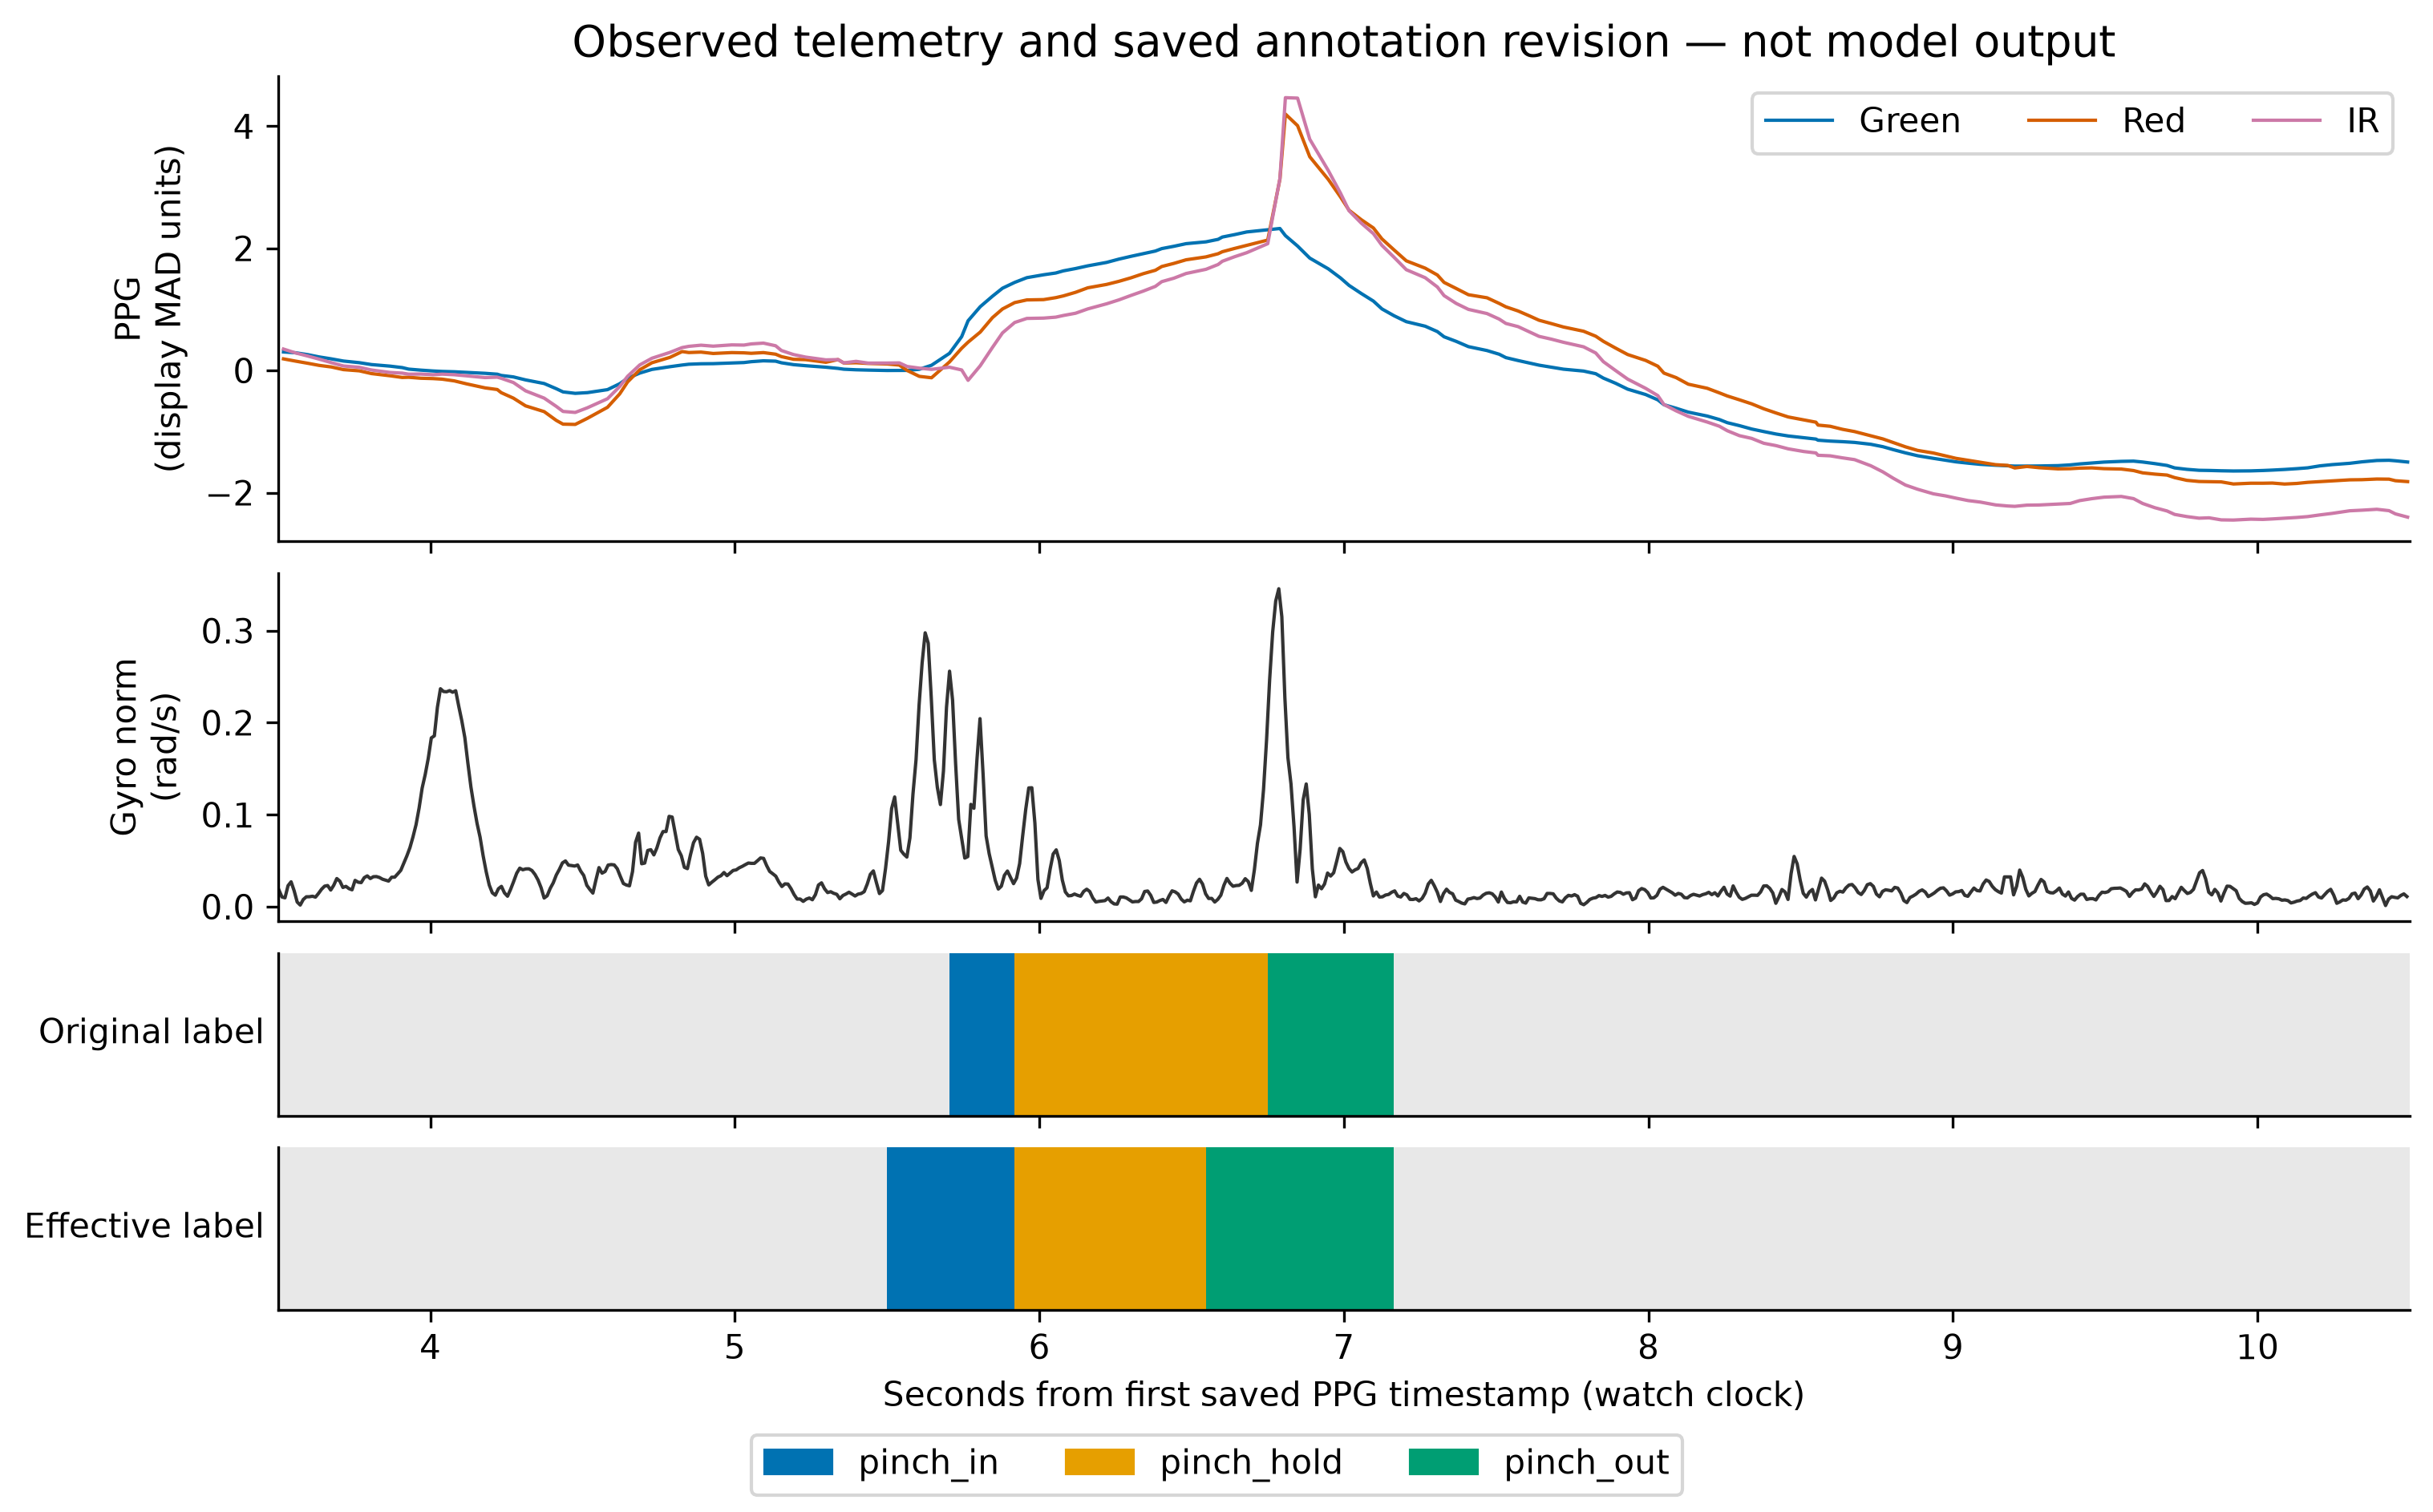
\includegraphics[width=1\linewidth,height=\textheight,keepaspectratio,alt={Saved optical and gyroscope data with original and effective row-label bands from a manually revised recording.}]{figures/annotation-telemetry.png}
\caption[Recorded PPG and gyroscope data with original and corrected labels]{Recorded PPG and gyroscope data from \nolinkurl{gesture-dataset-pinch_hold-2026-11-03T01-05-59.434Z}, with original and corrected label bands. Time is relative to the first PPG sample on the watch clock. For display only, each PPG channel is centred on its median and scaled by its MAD; gyroscope magnitude is in rad/s. No model output is shown.}\label{fig-annotation}
\end{widefigure}

\iffull
\subsect{Audit method}\label{audit-method}
\fi

\iffull
The audit reads every PPG and IMU file in the hand-labelled folder without changing anything. For each stream it hashes the ordered sensor columns, leaving out the label columns so that relabelled copies of the same data still match. The pair of PPG and IMU hashes identifies a source stream. We then match export names and recording IDs against the training and evaluation lists in each model manifest, and check each model file against its declared SHA-256.
\else
To find duplicates, we hashed each recording's ordered sensor columns, leaving out the labels, and used the pair of PPG and IMU hashes as the stream's identity. This catches exact copies but not partial overlaps.
\fi

\iffull
This finds exact duplicates only. Two crops of the same session, partial overlaps or a file saved in a different format would not match. Grouping by source is necessary for a clean split, but it cannot prove that days or sessions are independent, nor rule out repeated model selection on the evaluation data. The audit scripts, full inventory and figure sources are kept with the project artifacts (Section~\ref{limitations-and-reproducibility}).
\fi

\iffull
\subsect{Dataset identity findings}\label{dataset-identity-findings}
\fi

\iffull
The folder holds 37 exports totalling 127.918 minutes of PPG. Nine pairs of exports contain identical PPG and IMU streams under different names, which leaves 28 distinct streams and 98.080 minutes. This is total recording time after removing duplicates; it is not the same as independently collected sessions or no-gesture exposure. Six of the duplicate pairs carry pinch-hold and pinch-in names, and three carry supported and unlabelled names.
\else
The hand-labelled folder holds 37 exports (127.918 minutes of PPG), but nine pairs are identical streams under different names, leaving 28 distinct streams (98.080 minutes). Fourteen exports carry manual labels, which change the label of 4,931 PPG samples (Table~\ref{tab-audit}).
\fi

\iffull
Fourteen exports contain manual labels on PPG samples. Across all 37 exports, 4,931 PPG samples have a corrected label that differs from the original. That is a count of samples, not of editing actions or gesture events. Being in the folder does not prove a recording was reviewed, and an absent override does not prove it was not; reviews were not logged.
\fi

\begin{table}[t]
\centering\small
\caption[Hand-labelled folder audit]{Hand-labelled folder audit. Counts refer to exported files or exact stream pairs, not independent sessions.}\label{tab-audit}
\begin{tabularx}{\linewidth}{@{}>{\raggedright\arraybackslash}Xr>{\raggedright\arraybackslash}X@{}}
\toprule
\textbf{Quantity} & \textbf{Count} & \textbf{Note} \\
\midrule
Exported directories & 37 & Includes duplicates \\
Distinct stream pairs & 28 & Exact matches only \\
Duplicate pairs & 9 & Must share a split \\
Exports with PPG overrides & 14 & Review coverage unknown \\
PPG samples relabelled & 4,931 & Samples, not events \\
\bottomrule
\end{tabularx}
\end{table}

\iffull
For the hand-labelled pinch-in model, all 20 training and 8 evaluation IDs resolve to recordings in the folder. The two sets do not overlap, and no stream appears in both. So the duplicates we found did not leak into this particular split. Other median-model manifests use UUIDs that we could not map to the folder's metadata, so their splits remain unchecked.

\else
For the hand-labelled pinch-in model, the 20 training and 8 evaluation recordings share no stream, so these duplicates did not leak into its split.
\fi